\documentclass[8pt,a4paper,twocolumn]{scrreprt}

% Gib die Versuschsnummer an, um den entsprechenden Versuchsprotokoll zu laden
\newcommand{\versuchsnummer}{42}
\usepackage{Versuchs_Informationen}
\usepackage{style}


\begin{document}
\begin{titlepage}
\vspace*{2cm} 
  
  \centering
    
  % Versuchs-Titel
  {\LARGE\bfseries Protokoll zum Versuch \\[0.2cm]
  \textit{\versuchsname{\versuchsnummer}} \\[0.5cm] % Vielleicht wieder Anführungszeichen hinzufügen, leider Problem, da ein Leerzeichen falsch hinzugefügt wird.
  {\large (Versuch {\versuchsnummer})}
  \vspace{1.25cm}}

  % Tabelle mit Metadaten
  {\large
  \begin{tabular}{@{}rl@{}}
    Autor*innen:       & Annika Künstle,\\
                       & Finn Zeumer\\[0.5em]
    Versuchsbegleiter: & {\begleiter{\versuchsnummer}}\\[0.5em]
    Datum der Ausführung:& {\durchfuehrungsdatum{\versuchsnummer}}\\[0.5em]
    Abgabedatum:       & {\abgabedatum{\versuchsnummer}}\\[5em]
  \end{tabular}
  }
  \vfill


  \begin{tikzpicture}[remember picture,overlay]
    \node[opacity=1,inner sep=0] at (current page.center)
      {\includegraphics[width=\paperwidth,height=\paperheight]{hd-img/Titelhintergund_7_Page 2.png}};
  \end{tikzpicture}
  
\end{titlepage} 
% \onecolumn
\section{Fehlerrechnung}
Für die statistische Auswertung von $n$ Messwerten $x_i$ werden folgende Größen definiert \cite{errorSkript25}:
\begin{align}
    \bar{x} &= \frac{1}{n} \sum_{i=1}^{n} x_i \vphantom{\sqrt{\sum_i^n}^2} && \text{\textcolor{gray}{Arithmetisches Mittel}}\\
    \sigma^2 &= \frac{1}{n-1} \sum_{i=1}^{n} (x_i - \bar{x})^2 \vphantom{\sqrt{\sum_i^n}^2} && \text{\textcolor{gray}{Variation}}\\
    \sigma &= \sqrt{\frac{1}{n-1} \sum_{i=1}^{n} (x_i - \bar{x})^2} \vphantom{\sqrt{\sum_i^n}^2} && \text{\textcolor{gray}{Standardabweichung}}\\
    \Delta \bar{x} &= \frac{\sigma}{\sqrt{n}} = \sqrt{\frac{1}{n(n-1)} \sum_{i=1}^n(\bar x - x_i)^2} \vphantom{\sqrt{\sum_i^n}^2} && \text{\textcolor{gray}{Fehler des Mittelwerts}}\\
    \Delta f &= \sqrt{\left(\frac{\partial f}{\partial x} \Delta x\right)^2 + \left(\frac{\partial f}{\partial y} \Delta y\right)^2} \vphantom{\sqrt{\sum_i^n}^2} && \text{\textcolor{gray}{Gauß’sches Fehlerfortpflanzungsgesetz für $f(x,y)$}}\\
    \Delta f &= \sqrt{(\Delta x)^2 + (\Delta y)^2} \vphantom{\sqrt{\sum_i^n}^2} && \text{\textcolor{gray}{Fehler für $f = x + y$}}\\
    \Delta f &= |a| \Delta x \vphantom{\sqrt{\sum_i^n}^2} && \text{\textcolor{gray}{Fehler für $f = ax$}}\\
    \frac{\Delta f}{|f|} &= \sqrt{\left(\frac{\Delta x}{x}\right)^2 + \left(\frac{\Delta y}{y}\right)^2} \vphantom{\sqrt{\sum_i^n}^2} && \text{\textcolor{gray}{relativer Fehler für $f = xy$ oder $f = x/y$}}\\
    \sigma &= \frac{|a_{lit} - a_{gem}|}{\sqrt{\Delta a_{lit}^2 + \Delta a_{gem}^2}} \vphantom{\sqrt{\sum_i^n}^2} && \text{\textcolor{gray}{Berechnung der signifikanten Abweichung}}
\end{align}




\renewcommand{\contentsname}{Inhaltsverzeichnis}
\tableofcontents

% Lade die Versuchsnummer-spezifischen Informationen
\addcontentsline{toc}{chapter}{Messdaten} 
\label{Protokoll}

% \thispagestyle{empty}

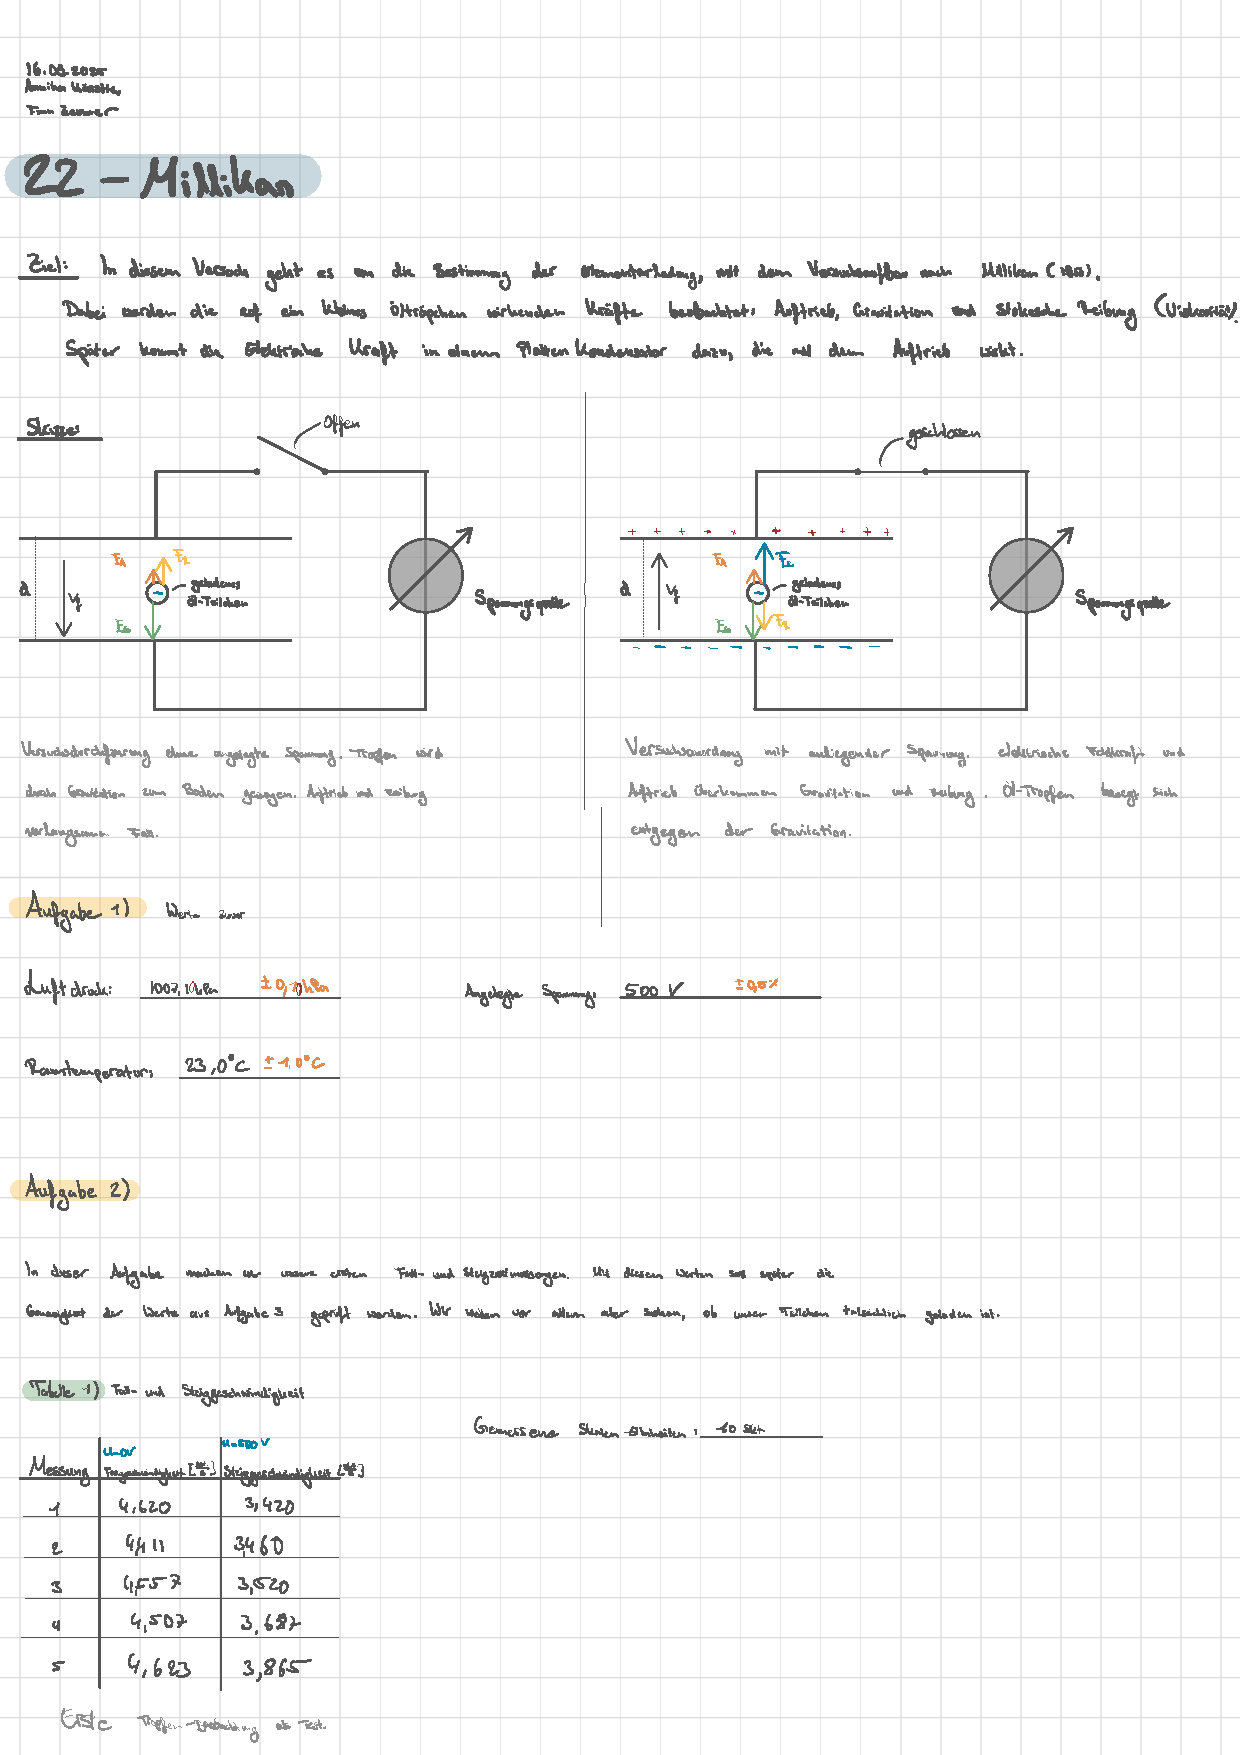
\includepdf[
  pages=1-3,               
  pagecommand={\thispagestyle{empty}} 
]{Protokolle/\versuchsnummer/Chapter/Messprotokoll.pdf}

\addcontentsline{lot}{table}{\protect\numberline{\thechapter.1} Pendellänge}
\addcontentsline{lot}{table}{\protect\numberline{\thechapter.2} (Vorläufige) Schwingdauer}
\addcontentsline{lot}{table}{\protect\numberline{\thechapter.3} GEnaue Bestimmung der Periodendauer}
\addcontentsline{lot}{table}{\protect\numberline{\thechapter.4} Bestimmung der Dämpfung}

\chapter{Einleitung}

\section{Aufgabe/Motivation}
\section{Physikalische Grundlage}
\cite{demtroeder17,skript25}


\chapter{Durchführung}
\label{ch:durchfuerung}

\section{Versuchsaufbau}

Der gesamte Versuch wurde auf einer optischen Bank durchgeführt, auf der Lampe, Kondensor, Linsenhalter, Filter, Blenden und Schirme in definierten Abständen montiert werden konnten. Die Justierung erfolgte jeweils so, dass die optische Achse aller Komponenten übereinstimmte. Als Lichtquelle diente eine Halogenlampe mit einstellbarem Kondensor. Zur Reduktion von Farbfehlern wurden Rot-, Blau- und Grünfilter eingesetzt.

\section{Messverfahren}

\subsection{Bestimmung der Parameter der achromatischen Linse}

Zunächst wurde die achromatisch korrigierte Linse (Achromat) zwischen Lampe und Schirm positioniert. Der Gegenstand (Testdia) wurde so ausgerichtet, dass ein scharfes Bild auf dem Schirm erschien. Für verschiedene Gegenstandsweiten $g$ wurden die zugehörigen Bildweiten $b$ bestimmt. In jedem Fall wurde vermerkt, ob das Bild reell oder virtuell und ob es aufrecht oder umgekehrt erschien. Aus den Messwerten lässt sich über \hyperref[eq:linsengleichung]{Gleichung \ref*{eq:linsengleichung}} die Brennweite bestimmen.

\subsection{Brennweitenmessung der bikonvexen Linse nach Bessel}

Zur Bestimmung der Brennweite der bikonvexen Linse $L_1$ wurde das Bessel-Verfahren angewendet. Der Abstand zwischen Gegenstand und Schirm wurde zu $L \approx 5f$ eingestellt. Anschließend wurde die Linse zwischen beiden Positionen verschoben, bis zwei Linsenstellungen mit scharfer Abbildung gefunden wurden. Aus dem Abstand $d$ dieser Positionen ergab sich die Brennweite nach \hyperref[eq:bessel]{Gleichung \ref*{eq:bessel}}. Zur Erhöhung der Genauigkeit wurde der Messvorgang mehrfach wiederholt.

\subsection{Untersuchung der chromatischen und sphärischen Aberration}

Die Messung der Brennweite wurde mit einem Rot- und einem Blaufilter wiederholt, um die chromatische Aberration zu untersuchen. Zusätzlich wurde die Linse einmal mit einer Lochblende und einmal mit einer Ringblende betrieben, um den Einfluss der sphärischen Aberration auf die Brennweite zu beobachten. Veränderungen des Abstandes $d$ zwischen den Bessel-Positionen deuten auf Unterschiede in der effektiven Brennweite hin.

\subsection{Aufbau und Untersuchung eines Mikroskops}

Für die Untersuchung des Mikroskops wurde eine Kombination aus Objektiv- und Okularlinse auf der optischen Bank aufgebaut. Als Objekt diente ein Kreuzgitter-Dia, das hinter einer Lampe mit Grünfilter positioniert wurde. Das Zwischenbild wurde in einem definierten Abstand zur Objektivlinse auf einem Schirm abgebildet, der eine Millimeterskala trug. Hinter dem Zwischenbild wurde das Okular in seiner Brennweite positioniert, sodass das Auge auf unendlich akkommodierte.

Die Vergrößerung wurde aus der Gitterstruktur des Zwischenbilds bestimmt. Anschließend wurde der einstellbare Spalt schrittweise verengt, bis die vertikalen Strukturen des Gitters gerade nicht mehr aufgelöst werden konnten. Aus der Spaltbreite und dem Abstand zum Objekt wurde der Öffnungswinkel berechnet, aus dem sich mit \hyperref[eq:auflösung]{Gleichung \ref*{eq:auflösung}} das Auflösungsvermögen ergab. Der Versuch wurde mit rotem und blauem Licht wiederholt, um den Einfluss der Wellenlänge auf die Auflösung zu überprüfen.

\begin{figure}[b!]
    \centering
    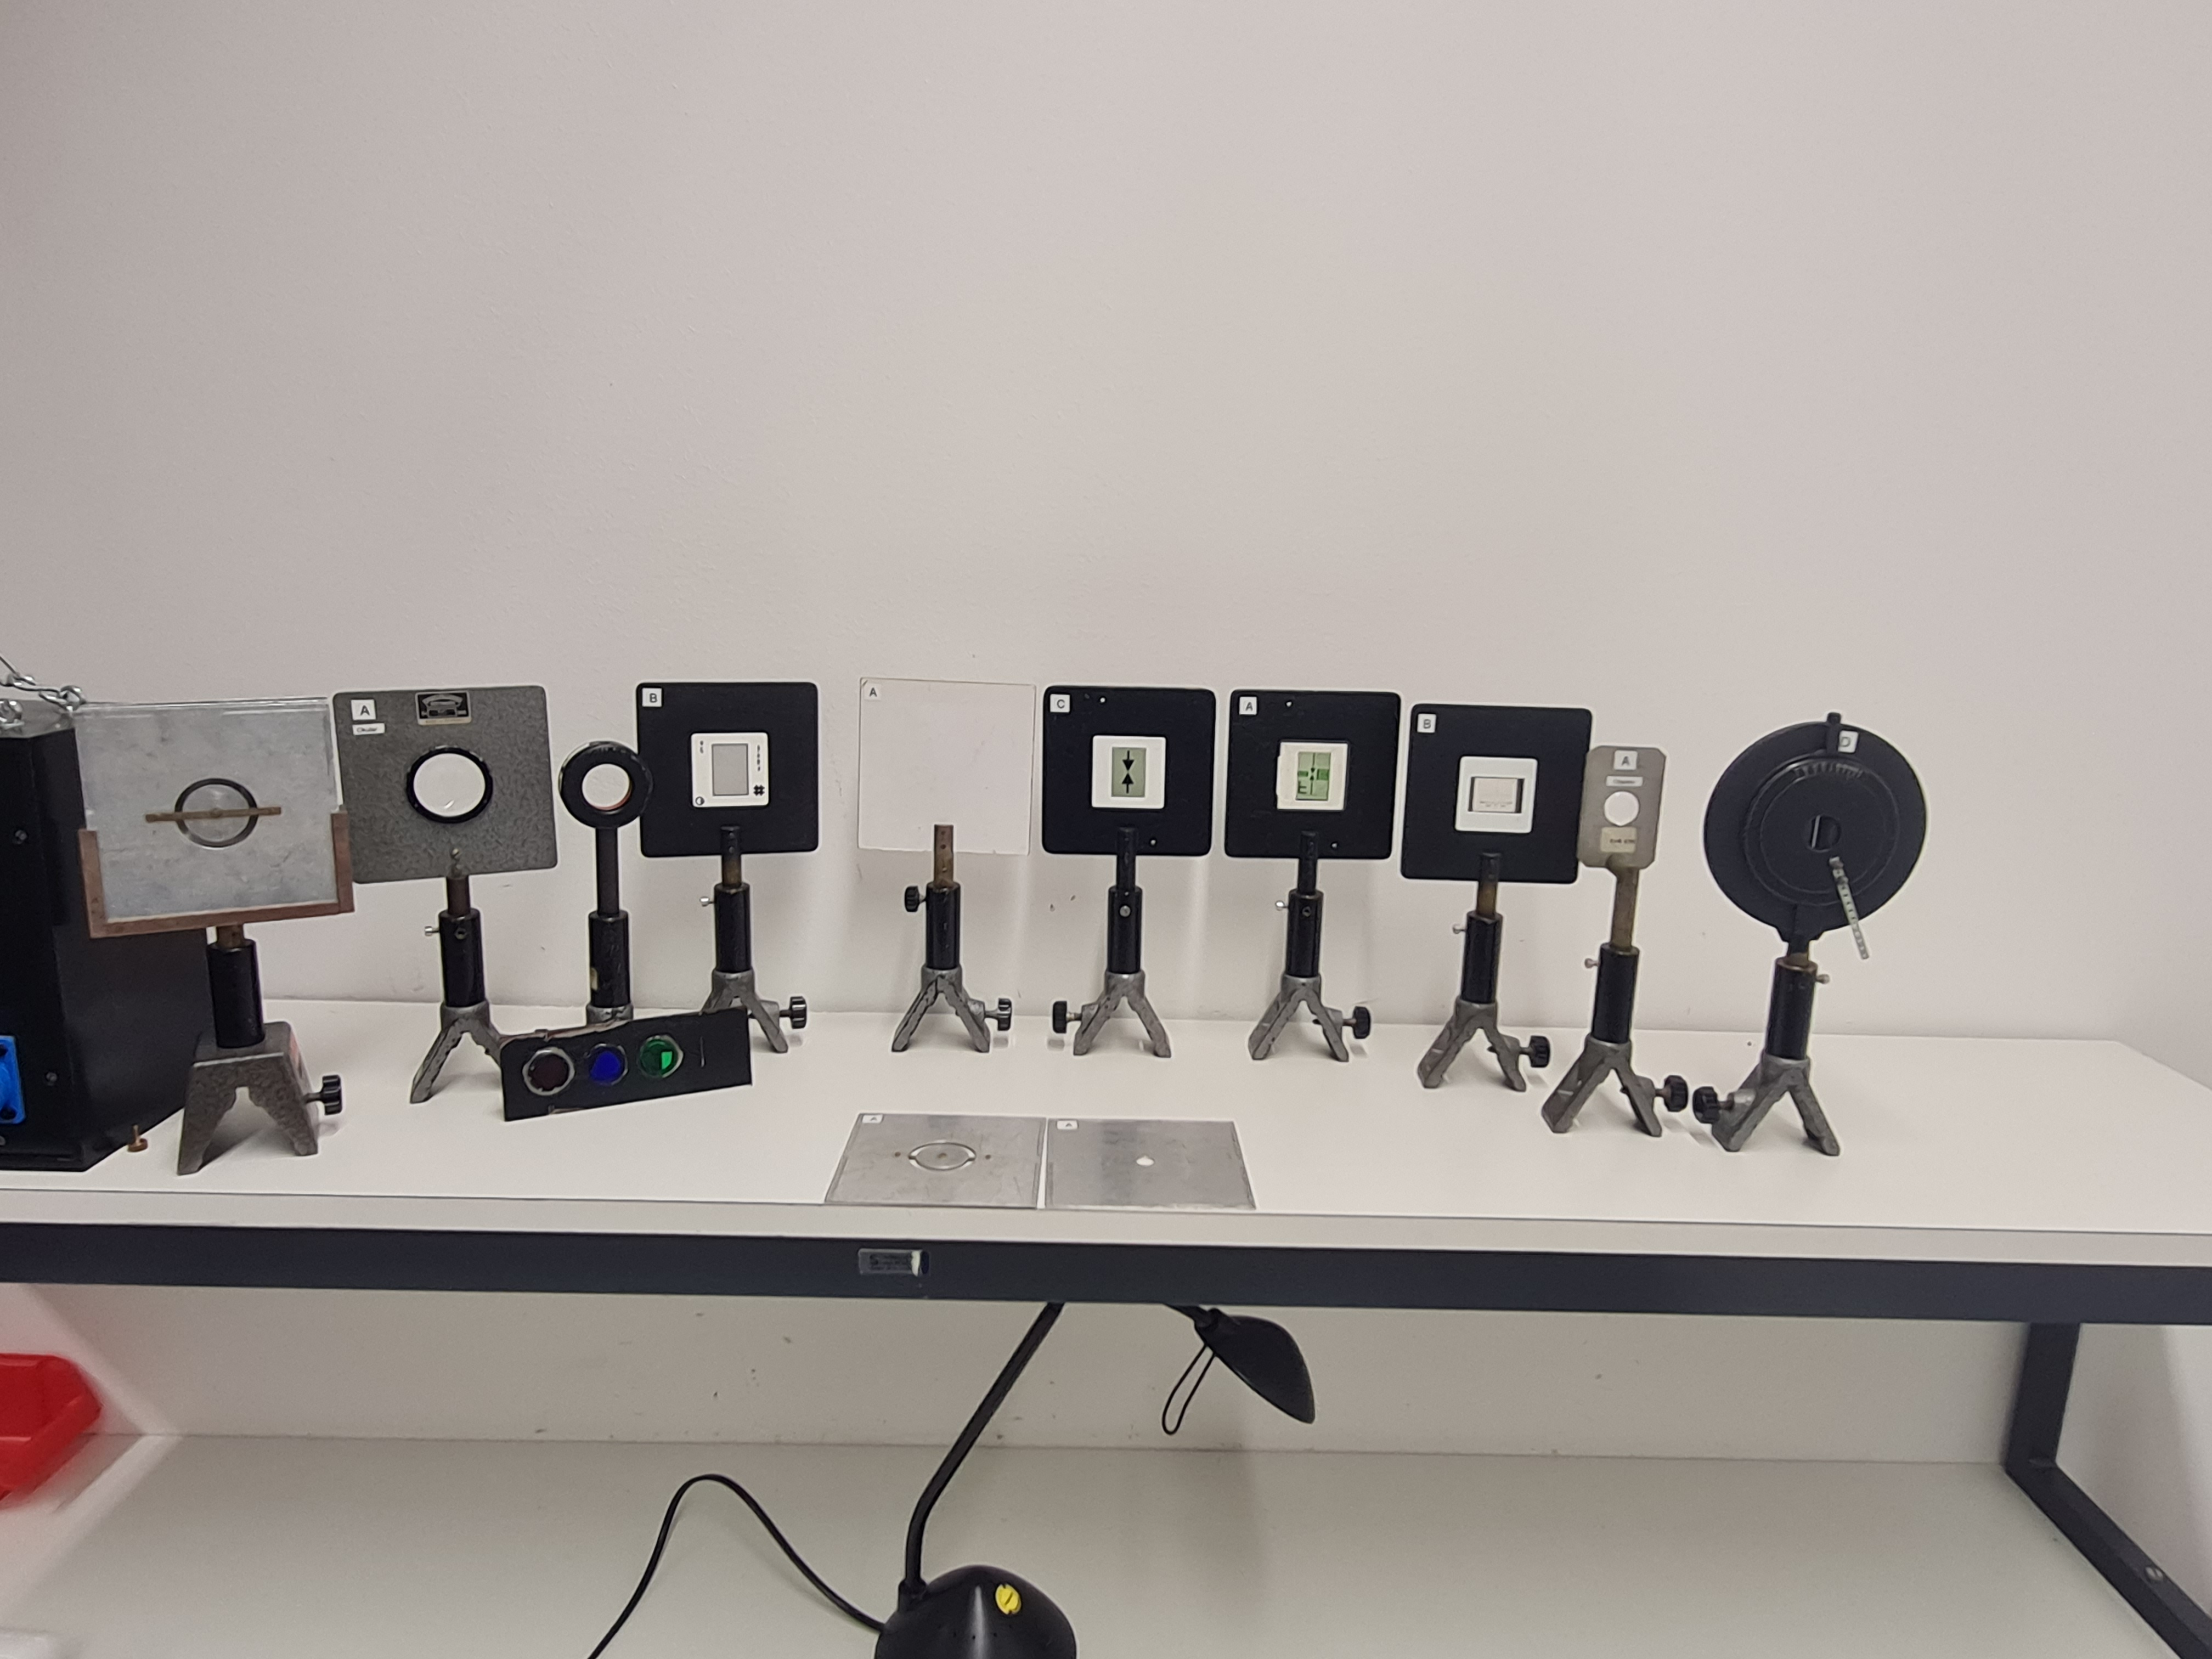
\includegraphics[width=\textwidth]{img/31/Versuchsbestandteile.jpg}
    \caption{Versuchsbestandteile}
\end{figure}

\onecolumn
\begin{figure}
    \centering
    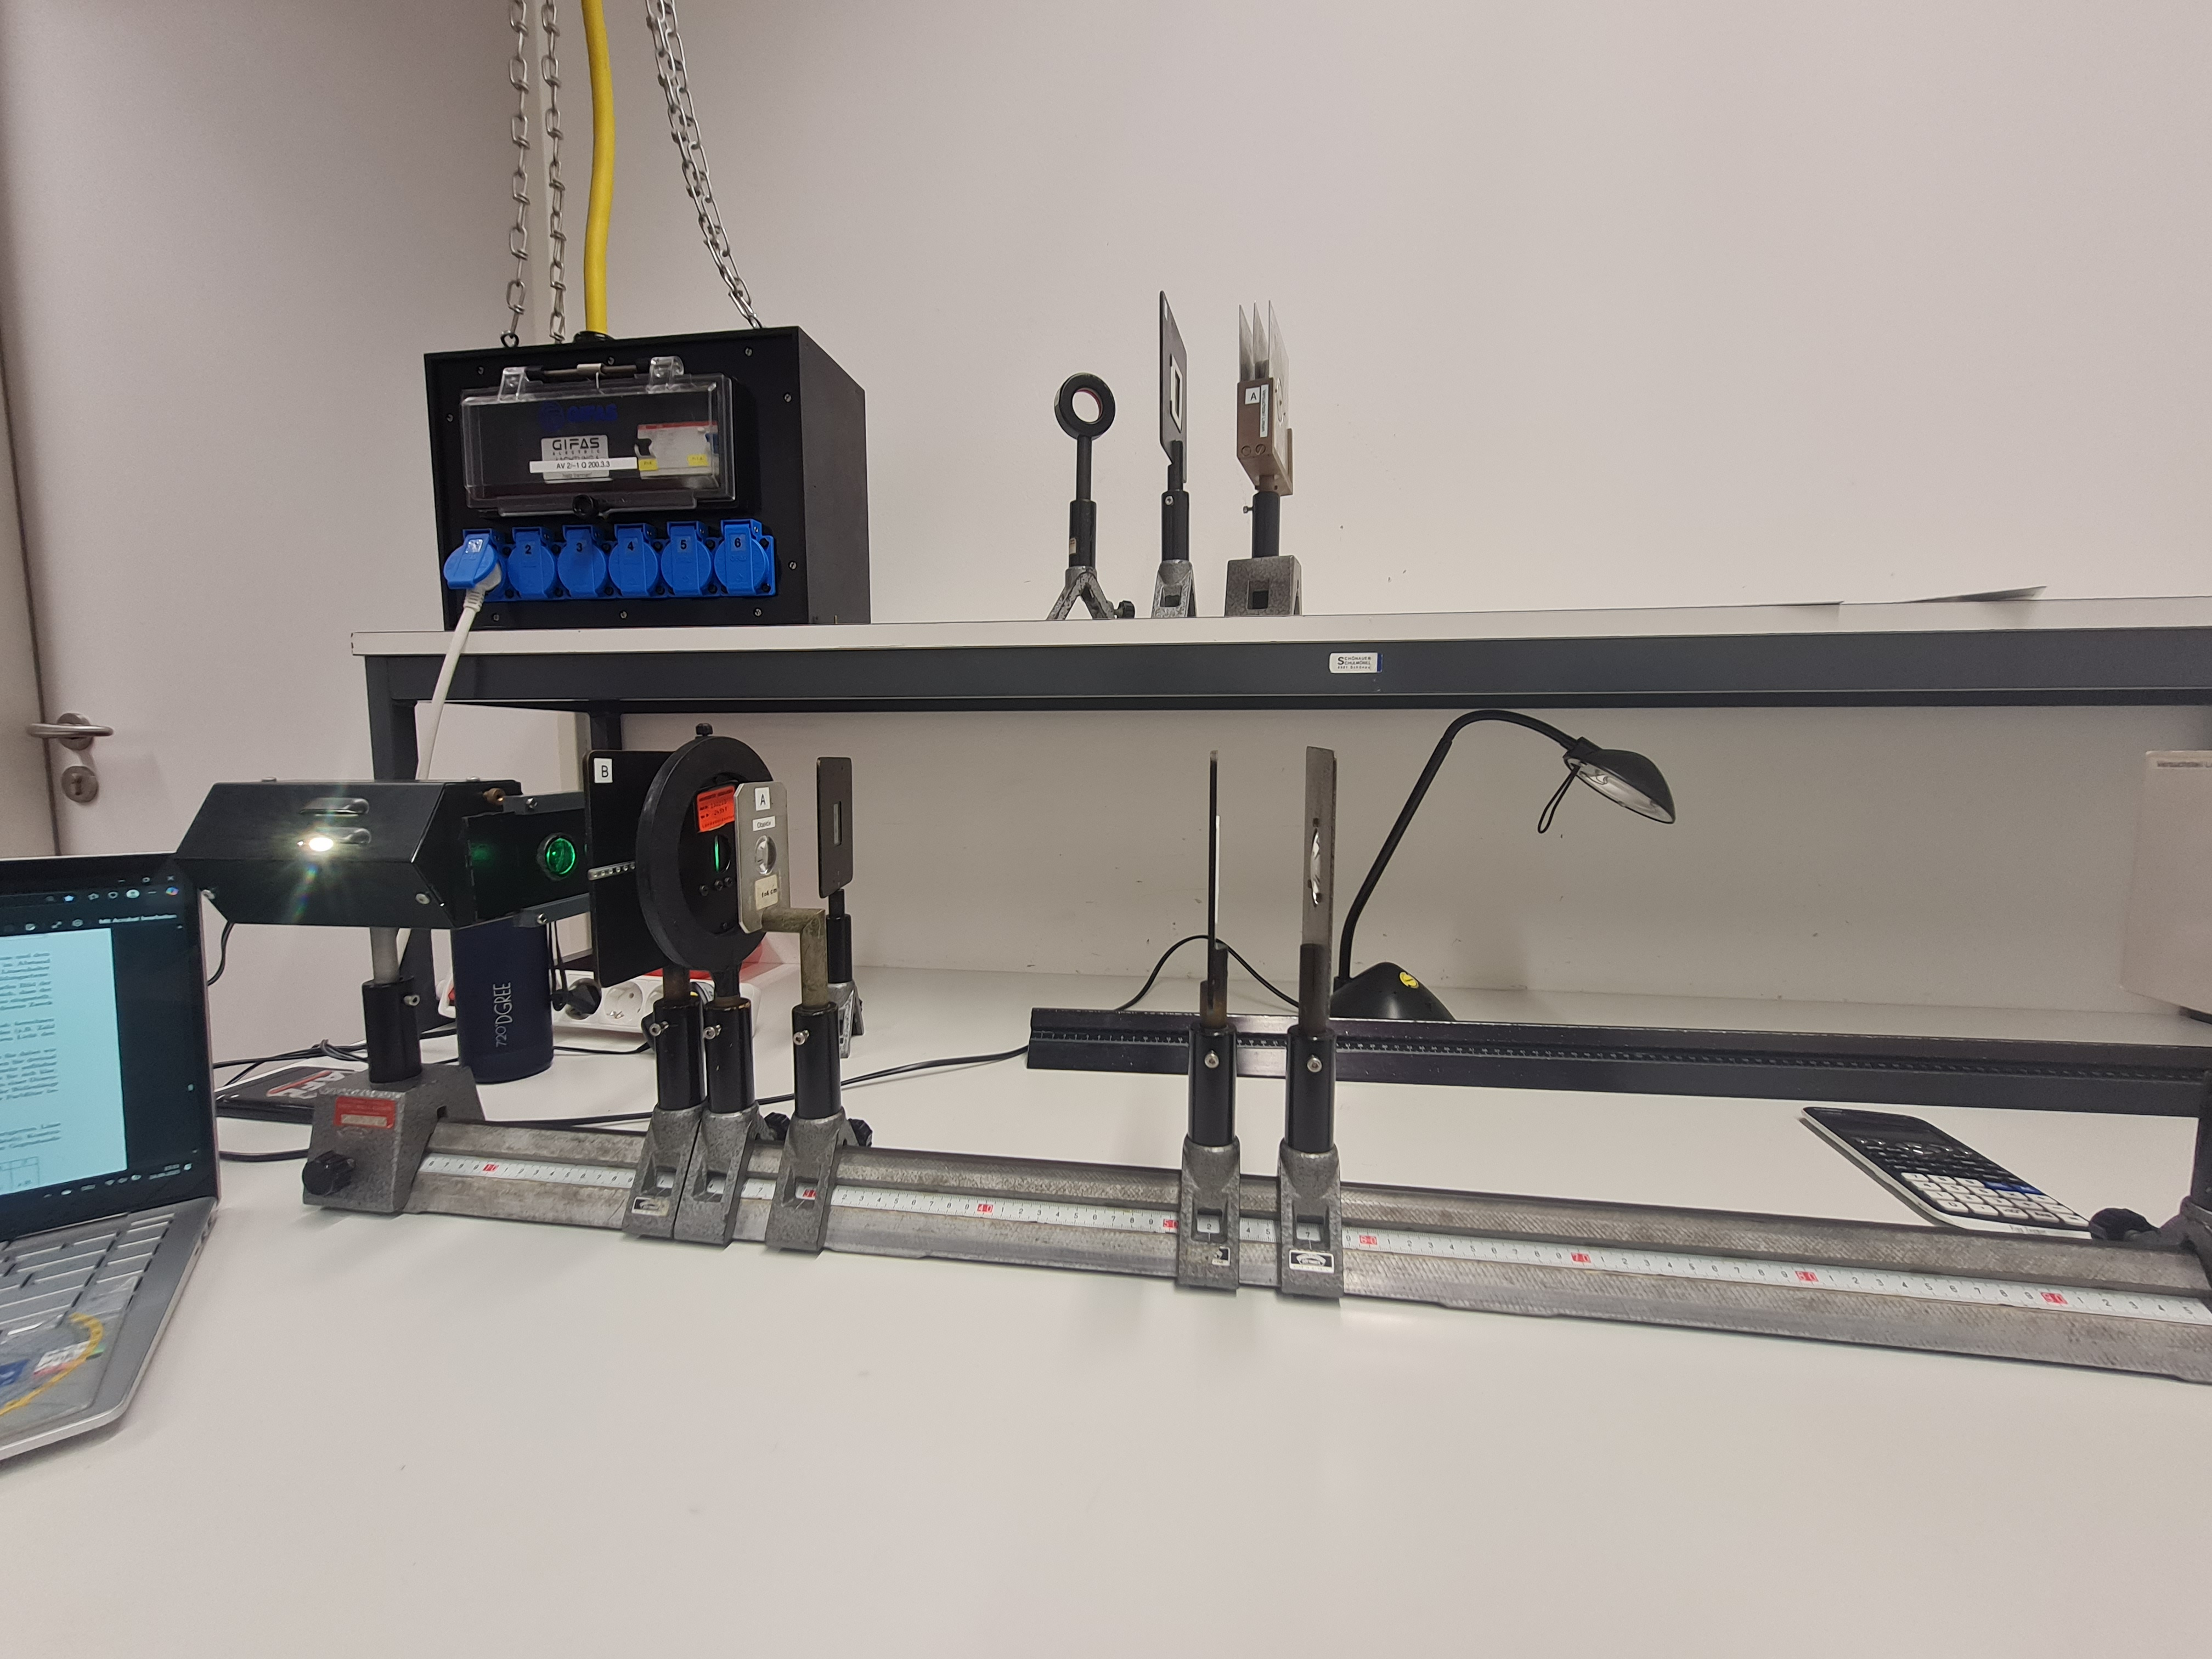
\includegraphics[width=\textwidth]{img/31/A2.jpg}
    \caption{Versuchsaufbau Aufgabe Gitter}
\end{figure}

\begin{figure}
    \centering
    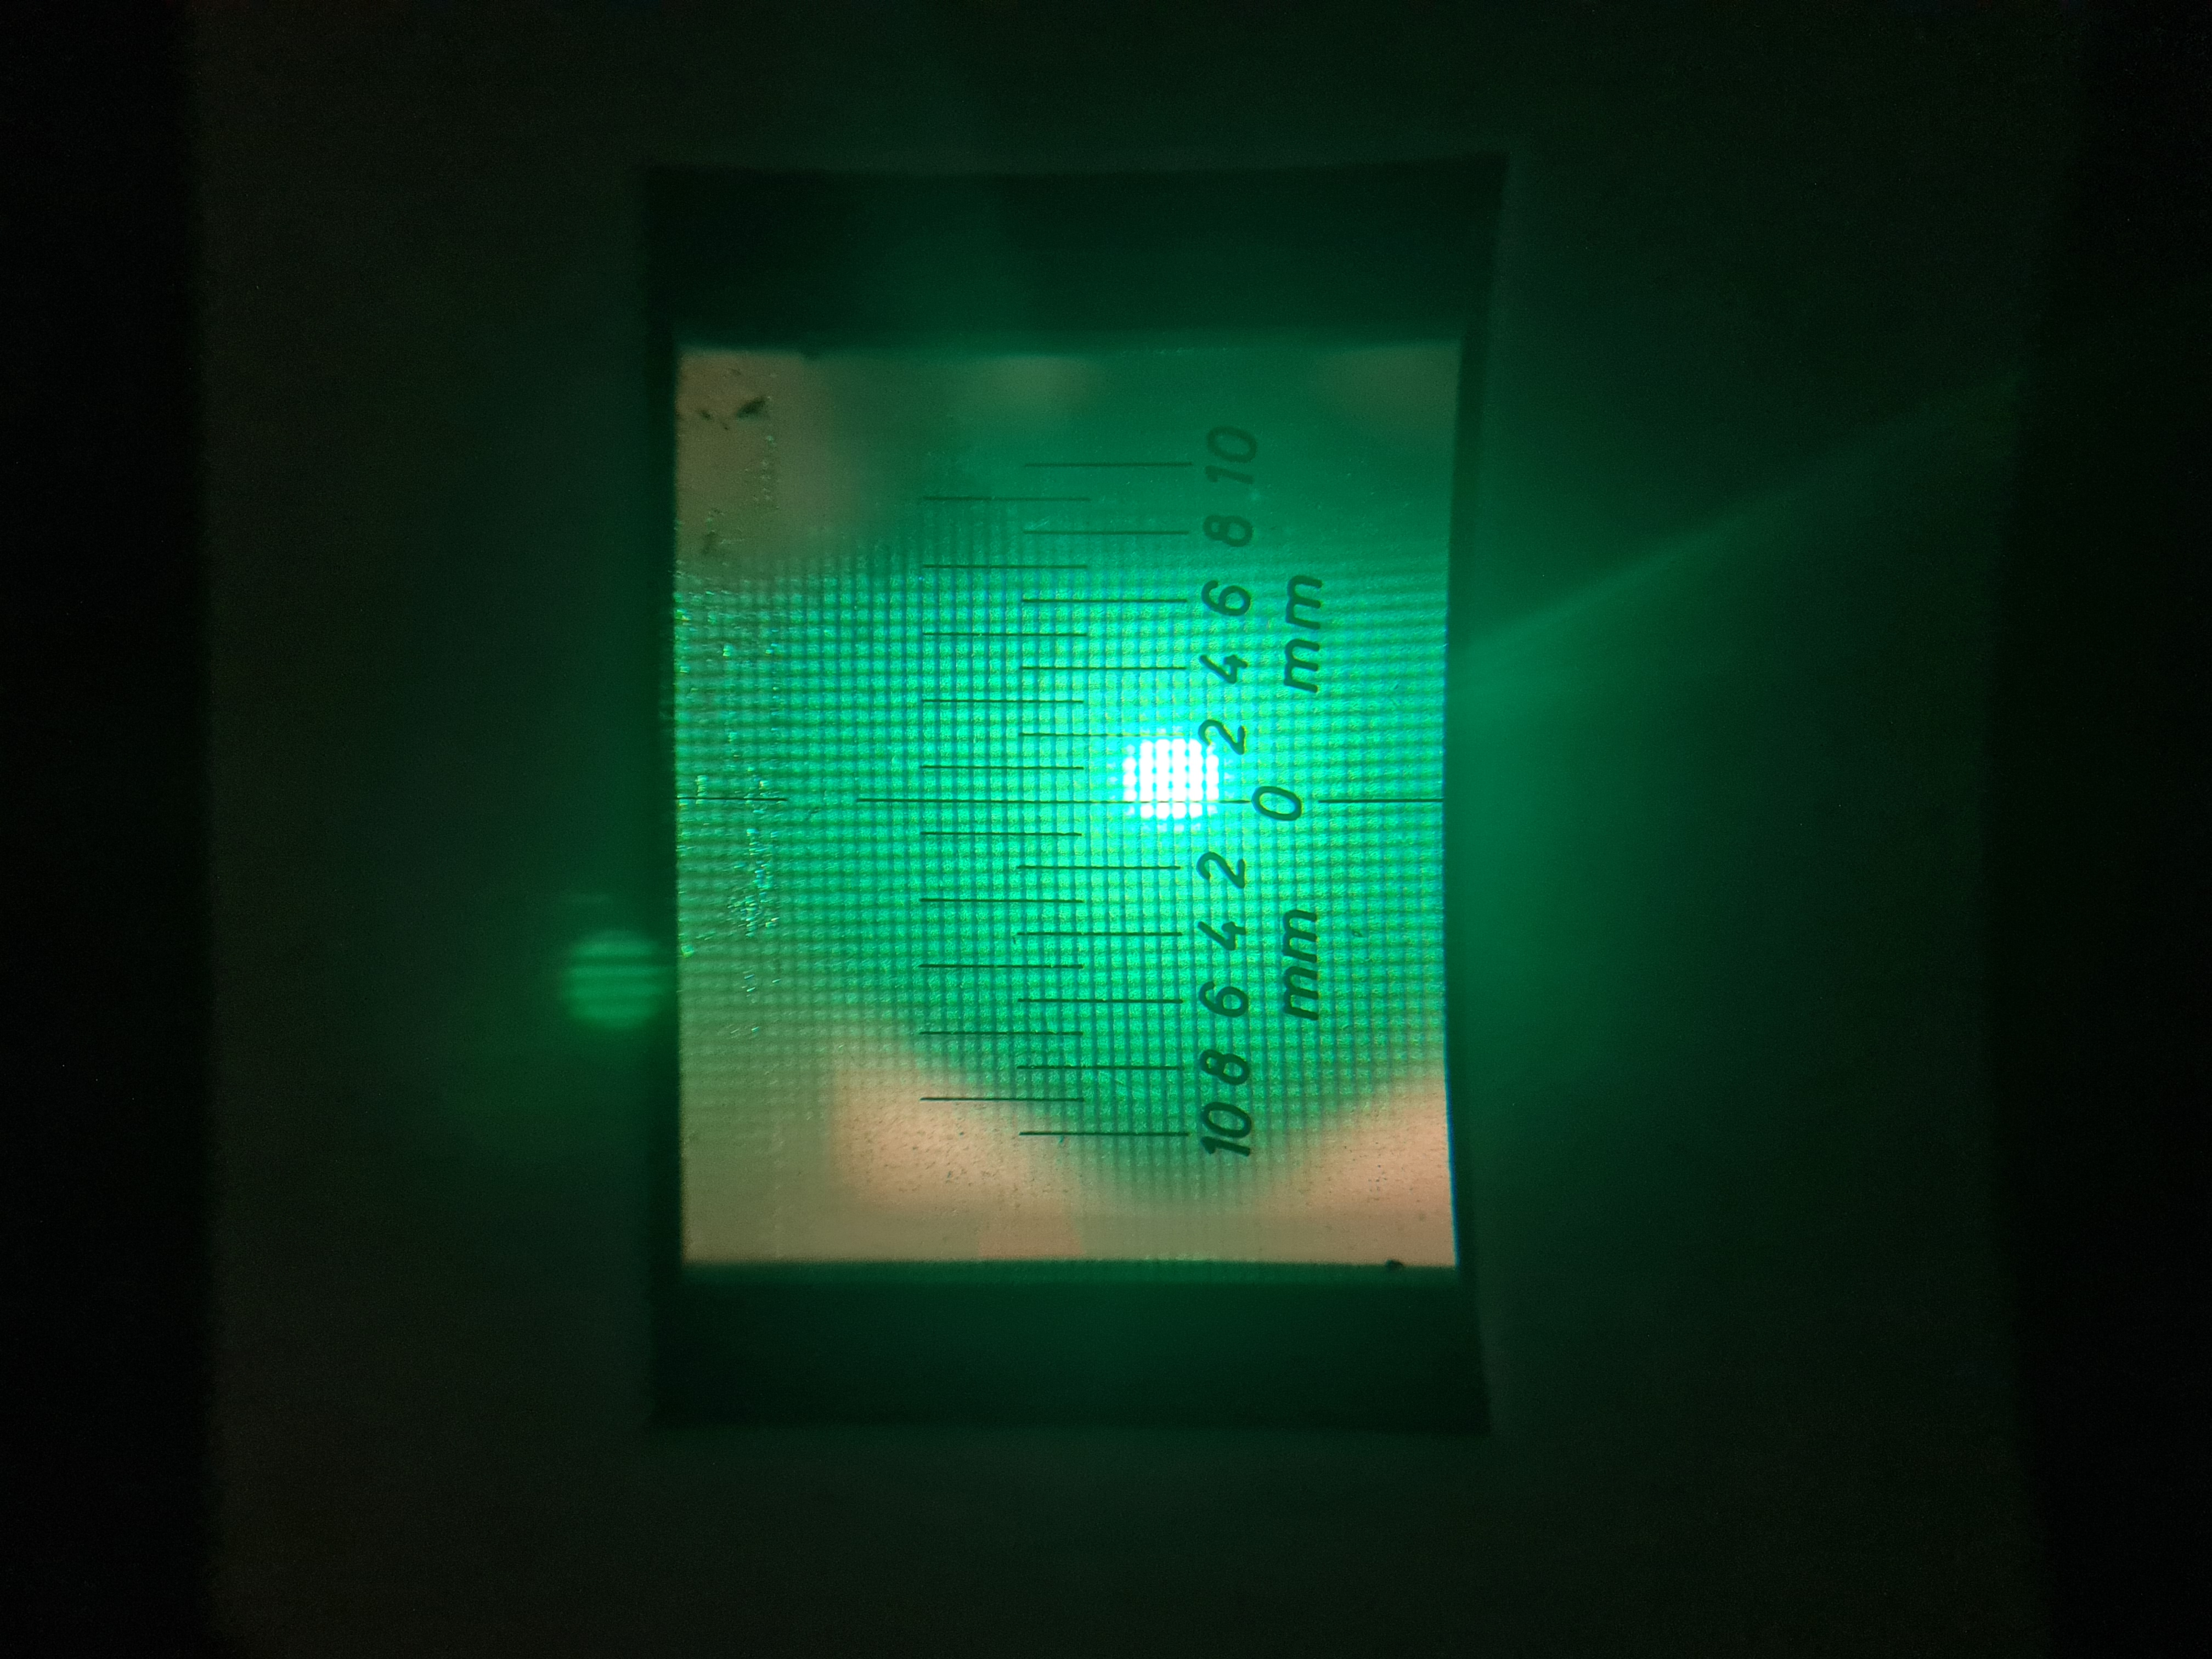
\includegraphics[width=\textwidth]{img/31/Gitter.jpg}
    \caption{Blich durch das Mikroskop auf das Gitter}
\end{figure}

\twocolumn
\onecolumn
\chapter{Auswertung}
\label{ch:auswertung}

\section*{Fehlerrechnung}
Für die statistische Auswertung von $n$ Messwerten $x_i$ werden folgende Größen definiert \cite{errorSkript25}:
\begin{align}
    \bar{x} &= \frac{1}{n} \sum_{i=1}^{n} x_i \vphantom{\sqrt{\sum_i^n}^2} && \text{\textcolor{gray}{Arithmetisches Mittel}} \label{eq:arithmetisches_mittel} \\
    \sigma^2 &= \frac{1}{n-1} \sum_{i=1}^{n} (x_i - \bar{x})^2 \vphantom{\sqrt{\sum_i^n}^2} && \text{\textcolor{gray}{Variation}} \label{eq:variation} \\
    \sigma &= \sqrt{\frac{1}{n-1} \sum_{i=1}^{n} (x_i - \bar{x})^2} \vphantom{\sqrt{\sum_i^n}^2} && \text{\textcolor{gray}{Standardabweichung}} \label{eq:standardabweichung} \\
    \Delta \bar{x} &= \frac{\sigma}{\sqrt{n}} = \sqrt{\frac{1}{n(n-1)} \sum_{i=1}^n(\bar x - x_i)^2} \vphantom{\sqrt{\sum_i^n}^2} && \text{\textcolor{gray}{Fehler des Mittelwerts}} \label{eq:fehler_mittelwert} \\
    \Delta f &= \sqrt{\left(\frac{\partial f}{\partial x} \Delta x\right)^2 + \left(\frac{\partial f}{\partial y} \Delta y\right)^2} \vphantom{\sqrt{\sum_i^n}^2} && \text{\textcolor{gray}{Gauß’sches Fehlerfortpflanzungsgesetz für $f(x,y)$}} \label{eq:gauss_fehlfortpflanzung} \\
    \Delta f &= \sqrt{(\Delta x)^2 + (\Delta y)^2} \vphantom{\sqrt{\sum_i^n}^2} && \text{\textcolor{gray}{Fehler für $f = x + y$}} \label{eq:fehler_summe} \\
    \Delta f &= |a| \Delta x \vphantom{\sqrt{\sum_i^n}^2} && \text{\textcolor{gray}{Fehler für $f = ax$}} \label{eq:fehler_proportional} \\
    \frac{\Delta f}{|f|} &= \sqrt{\left(\frac{\Delta x}{x}\right)^2 + \left(\frac{\Delta y}{y}\right)^2} \vphantom{\sqrt{\sum_i^n}^2} && \text{\textcolor{gray}{relativer Fehler für $f = xy$ oder $f = x/y$}} \label{eq:relativer_fehler} \\
    \sigma &= \frac{|a_{lit} - a_{gem}|}{\sqrt{\Delta a_{lit}^2 + \Delta a_{gem}^2}} \vphantom{\sqrt{\sum_i^n}^2} && \text{\textcolor{gray}{Berechnung der signifikanten Abweichung}} \label{eq:signifikante_abweichung}
\end{align}

\twocolumn

\section{Molarextintion über die Lambert-Gerade}
Für folgende Rechnung liegen die Werte der Tabelle 1 des \hyperref[Protokoll]{Protokolls} zugrunde. Aus diesen soll die Molarextintion über die Lambert-Gerade bstimmt werden. Hierfür wird die gemessene Intensität gegen die Schichtdicke des Kaliumpermanganat geplottet. Dies wird auf halblogarithmischen papier gemacht. Zunächst muss die Ungenauigkeit der Intensität bestimmt werden, dies geschieht über die \hyperref[eq:gauss_fehlfortpflanzung]{Gauß'sche Fehlerfortpflanzung (\ref*{eq:gauss_fehlfortpflanzung})} der \hyperref[eq:correction]{Gleichung \ref*{eq:correction}}:
\begin{equation}
    \hspace{-0.25cm}
    \frac{\Delta I_{\text{korr}}}{I_{\text{korr}}} = \sqrt{\left(\frac{\Delta I}{I}\right)^2 + \left(\frac{2 \Delta D_{\text{mK}}}{D_{\text{mK}}}\right)^2 + \left(\frac{2 \Delta D_{\text{oK}}}{D_{\text{oK}}}\right)^2}
\end{equation}


Dies ist der Fehler der längsten Küvette (25cm). Die Abbildunsggröße betrug dabei $(22,0 \pm 1,4) \mathrm{mm}$. Die Intensität ist der Mittelwert der 5 Einzelmessungen Somit kommt man auf eine Ungenauigkeit von:
\begin{equation}
    I_{\text{korr}} = 280 \pm 60
\end{equation}

Die Werte der Tabelle 1 des pp nochmal schön aufgetragen, mit korrigierten \hyperref[eq:fehler_mittelwert]{Fehler des Mittelwerts (\ref*{eq:fehler_mittelwert})}:
\begin{table}[b!]
    \onecolumn
    \centering
    \begin{tabular}{l | ccccc}
    \hline
    Nr. & Probe 1 & Probe 2 & Probe 3 & Probe 4 & Probe 5 \\
    \hline
    1 & 57986,15 & 42025,17 & 20706,55 & 3785,81 & 238,52 \\
    2 & 58064,89 & 42039,61 & 20728,90 & 3785,01 & 236,01 \\
    3 & 58051,22 & 42059,49 & 20698,69 & 3783,42 & 234,55 \\
    4 & 58091,77 & 42055,26 & 20696,26 & 3770,97 & 236,08 \\
    5 & 58038,11 & 42051,74 & 20700,11 & 3782,10 & 234,51 \\
    \hline
    $\bar{x} \pm \Delta \bar{x}$ & 58046 $\pm$ 16 & 42046 $\pm$ 6 & 20706 $\pm$ 5 & 3781,5 $\pm$ 2,4 & 235,9 $\pm$ 0,7 \\
    \hline
    \end{tabular}
    \caption{Messwerte der fünf Proben mit Mittelwert und Standardfehler des Mittelwerts (SEM).}
    \twocolumn
\end{table}

Die Ergebnisse sind in \hyperref[fig:g_l]{Abbildung \ref*{fig:g_l}} dargestellt. Mit den \hyperref[eq:beer]{Gleichungen \ref*{eq:beer} und \ref*{eq:combined}} ergibt sich:

\begin{equation}
\frac{\lg(I_0) - \lg(I(l))}{l} = k'
\end{equation}

Damit sind die Steigungen der beiden geraden:
\begin{align}
    {k_A}' &= \frac{\lg(60\,000) - \lg(95)}{28,85\mathrm{cm}} = -0,09707 \, \frac{1}{\mathrm{cm}}\\
    {k_F}' &= \frac{\lg(58\,056) - \lg(220)}{22,5\mathrm{cm}} = -0,10762 \, \frac{1}{\mathrm{cm}}
\end{align}

Damit ergibt sich:
\begin{equation}
\boxed{
    k' = (0,0971\pm 0,0106) \, \frac{1}{\mathrm{cm}}
}
\end{equation}

Nun \hyperref[eq:beer]{Gleichung \ref*{eq:beer}} nach $\epsilon$ umformen und \hyperref[eq:gauss_fehlfortpflanzung]{Gauß'sche Fehlerfortpflanzung (\ref*{eq:gauss_fehlfortpflanzung})} anwenden:
\begin{equation}
    \Delta \epsilon = \frac{\Delta k'}{c}
\end{equation}

Daraus ergibt sich bei einer Konzentration von $c = 5 \cdot 10^{-5} \, \mathrm{\frac{mol}{l}}$:
\begin{equation}
\boxed{
    \epsilon = (1900 \pm 200) \, \mathrm{\frac{cm^2}{mol}}
}
\end{equation}

\onecolumn
\begin{figure}
    % \hspace{-2.2cm}
    \includegraphics[width=1\textwidth]{img/34/g1--34–Spektralfotometrie.pdf}
    \caption{Ausgelichsgerade (blau) und Fehlergerade (orange) der Messwerte aus Tabelle 1 für das Lambert-Verfahren}
    \label{fig:g_l}
\end{figure}
\twocolumn

\section{Molarextintion über die Beer-Gerade}
In dieser Sektion wird die molare Extinktion mithilfe der Beer’schen Gerade berechnet. Dazu werden die Intensitäten aus Tabelle 2 des \hyperref[Protokoll]{Protokolls} als Funktion der Konzentration \( c \) der verwendeten Lösung dargestellt. Die Konzentrationen ergeben sich aus den Messprotokollangaben; die entsprechenden Werte sind bereits im Praktikumsskript enthalten \cite{skript25}. Zusätzlich muss für jede Konzentration der zugehörige Fehler bestimmt werden.

Der allgemeine Ausdruck für den Fehler \(\Delta c_i\) lautet:

\begin{equation}
\Delta c_i = \tilde{c} \frac{1}{V_{\text{ges}}^2}
\left(
V_0^2 \sum_{j=1}^{i} \Delta V_j^2 + (V_{\text{ges}} - V_0)^2 \Delta V_0^2
\right)^{\frac{1}{2}}
\end{equation}

Dabei ist \(\tilde{c} = 10^{-3}\,\text{mol/l}\) die Konzentration der Kaliumpermanganat-Lösung in der Bürette, mit der die Küvette befüllt wird. Der Volumenfehler \(\Delta V_j\) ist dem Messprotokoll zu entnehmen.

Das Gesamtvolumen \(V_{\text{ges}}\) der Lösung ergibt sich zu:

\begin{equation}
V_{\text{ges}} = \sum_{j=0}^{i} V_j
\end{equation}

Die Ergebnisse sind \hyperref[tab:beer]{tabellarisch \ref*{tab:beer}} festgehalten.
\begin{table}[!ht]
    \centering
    \begin{tabular}{l | c | c}
        \toprule
        Nr. & $c_i {\mathrm{\frac{mol}{l}} \cdot 10^{-4}}$ & Itensität \\
        \hline
        1 & $0,0 \pm 0,0$ & $57830 \pm 16$ \\
        2 & $0,63 \pm 0,06$ & $31597 \pm 5$ \\
        3 & $1,25 \pm 0,07$ & $16905 \pm 8$ \\
        4 & $2,5 \pm 0,07$ & $4342 \pm 4$ \\
        5 & $5 \pm 0,04$ & $234,86 \pm 1,05$ \\         
        \bottomrule
    \end{tabular}
    \label{tab_beer}
    \caption{Ergebniss der Konzentrationen und der gemessenen Itensitäten.}
\end{table}

Aus \hyperref[fig:g_2]{Abbildung \ref*{fig:g_2}} sind die Steigungen 
\begin{align}
    m_A &= -6950,61728 \, \mathrm{\frac{l}{mol}}\\
    m_F &= -11523,77183 \, \mathrm{\frac{l}{mol}}
\end{align}

somit ergibt sich eine Steigungen:
\begin{equation}
\boxed{
    m = -(7000 \pm 5000) \, \mathrm{\frac{l}{mol}}
}
\end{equation}

Für das $\epsilon$ ergibt sich über
\begin{equation}
\epsilon_B = \frac{s}{l} 
\end{equation}

und seinem Fehler 
\begin{equation}
\Delta \epsilon_B = \frac{\Delta  s}{l} 
\end{equation}

folglich bei einer dicke von $l = 1,5$ cm:

\begin{equation}
\boxed{
    \epsilon_B = (5000 \pm 3000) \cdot 10^3 \mathrm{\frac{cm^2}{mol}}
}
\end{equation}

\section{Abweichung der Ergebnisse}
Zuletzt wird die \hyperref[eq:signifikante_abweichung]{signifikante Abweichung (\ref*{eq:signifikante_abweichung})} berehnet:
\begin{equation}
    \frac{\left| \epsilon_L - \epsilon_B \right|}{\sqrt{(\delta \epsilon_L)^2 + (\delta \epsilon_B)^2}} = 1,03\sigma
\end{equation}

\onecolumn
\begin{figure}
    % \hspace{-2.2cm}
    \includegraphics[width=1\textwidth]{img/34/g2--34-Spektralfotometrie.pdf}
    \caption{Ausgelichsgerade (blau) und Fehlergerade (orange) der Messwerte aus Tabelle 1 für das Lambert-Verfahren}
    \label{fig:g_2}
\end{figure}
\twocolumn
\chapter{Disskusion}
\label{sc:dis}
\section{Zusammenfassung}

\section{Disskusion}

\section{Kritik}
\onecolumn
\chapter{Veruschsaufbauten}
Im folgenden sind die verschiedenen Veruschsaufbauten mit ihren Maßen aufgelistet. Werte, die mit einem Strich versehen sind, sind gemessene Werte. Jene ohne Strich sind berechnete Werte. Die Maßstäbe sind möglichst präzise gesetzt.

\begin{figure}[!ht]
    \section{Maße der Rollebene}
    \centering
    \includegraphics[width=1\textwidth]{img/15/Maße-RollEbene.pdf}
    \caption{Gemessene Längen der Abrollebene, zudem der Berechnete Neigungswinkel und die berechnete Starthöhe.}
    \label{fig:maße_re}
\end{figure}

\begin{figure}[!ht]
    \section{Maße der LS Messung Beschelunigung}
    \centering
    \includegraphics[width=1\textwidth]{img/15/Aufbau2.pdf}
    \caption{Gemessene Längen der Abrollebene, zudem der Berechnete Neigungswinkel und die berechnete Starthöhe.}
    \label{fig:maße_2}
\end{figure}

\begin{figure}[!ht]
    \section{Maße der LS Messung Geschwindigkeit}
    \centering
    \includegraphics[width=1\textwidth]{img/15/Aufbau3.pdf}
    \caption{Gemessene Längen der Abrollebene, zudem der Berechnete Neigungswinkel und die berechnete Starthöhe.}
    \label{fig:maße_3}
\end{figure}

\begin{figure}[!ht]
    \section{Maße der Messzylinder}
    \centering
    \includegraphics[width=0.85\textwidth]{img/15/Zylindermasse.pdf}
    \caption{3D-Rendering mit den vermessene Größen der Zylinder eingezeichnet (Maßstabsgetreu).}
    \label{fig:zylinder_masse}
\end{figure}
\twocolumn

\listoffigures
\cleardoublepage

\listoftables
\cleardoublepage

% Beispielhafte Zitierung, damit keine Fehlermeldeung entsteht lol
\cite{demtroeder17}

\bibliographystyle{alpha}
\bibliography{Literaturverzeichnis}

\end{document}